We have implemented \cf in full with the exception of the intra-channel interference management component -- current small cell software for the cells we used does not support some of the required standard LTE feature (see Section~\ref{sec:implementation} for details). A \cf access point has currently been operational for several months serving more than 10 users with no broadband connection as identified by a local charity. The need for serving under-privileged population highlights one of the potential use-cases of a long-range, unlicensed, low-cost cellular network. Our users can access the Internet through our gateway using standard LTE clients inside their homes without special outdoor equipment or antennas. In agreement with the requirements identified in Section~\ref{sec:requirements}, the network range is around 1km and all users experience rates above 1Mbps. Due to privacy restrictions, we are unable to share any performance numbers related to these users. 

Our evaluation covers the main novel components of the system, i.e., channel selection and interference management, through a series of experiments on our testbeds and in simulations. Simulations are used to evaluate the interference management component which we are unable to implement -- yet, simulation parameters such as potential inaccuracies of our sensing mechanisms, or interference due to control signaling are guided by our testbed measurements. To this end, we are confident about the realism of our simulated results.


%% Our evaluation focuses on two main aspects of \cf. First, we evaluate
%% the feasibility of our design based on experiments with off-the-shelf and custom LTE equipment that we have built. 
%% Second,  we perform a large-scale performance evaluation through simulations. 
%% We use our feasibility study to guide our modeling of interference during the large-scale simulations 
%% by feeding the measurement results into the simulator.



%% \subsection{Test-bed evaluation}
%% \label{sec:testbed}


%% Our test-bed evaluation comprise four experiments. 
%% First, we implement the channel selection client and we show that it satisfies the TVWS regulatory requirements. 
%% Second, we examine the effect of signaling and control channel interference on our design. 
%% Third, we examine whether CQI reports provide an accurate indicator of channel quality. 
%% Finally, we implement a PRACH detector using our software-defined radio to evaluate its complexity.


\subsection{Implementation Details}
\label{sec:implementation}

We implement our architecture using IP Access E40 small cells~\cite{ipa}. The small cell operates on 3GPP band 13, which we can use in our area. 
The transmit power of the small cell is 23 dBm. We further use Amphenol directional antenna with 7dBi gain and about 120 degree sector width. 

Channel selection is implemented on a PC. We interface and test it with a certified Nominet spectrum database~\cite{nominet}. 
We are unable to implement the interference management controler on our current small cells due to lack of software support for the X2 interface and CQI aperiodic mode 3-0 (sub-band level report). Instead, we implement the full component within ns-3 simulator and evaluate its basic mechanisms in a test-bed.

The mobile client used in the experiment is based on a Qualcomm MDM9625 chipset. 
The client's transmit power is limited to 20dBm, as per TVWS specifications. 
We use QXDM to get CQI information and other internal signaling information from the mobile client.

We have also built a custom access point on a software designed radio (SDR) that supports a limited set of LTE features; 
our SDR access point is fully LTE compliant at the PHY level, which we have verified using commercial LTE test equipment.
We use the custom access point to introduce controlled interference and evaluate the complexity of the PRACH detector;
we are otherwise unable to achieve these using the commercial small cell. 

Measurements without SDR are performed outdoors. Measurements with SDR are performed indoors as the SDR was not equipped with the adequate power amplifier to reach the same range. 

%All experiments are performed indoors because of limited transmit powers. 
%The overall area of the experiments is 50m $\times$ 25m and it includes an elevator shaft, staircases and a glass atrium %in the middle of the floor. 


%% \subsubsection{Out-of-band Interference}
%% {\bf XXXX the following appears too esoteric -- would be nice to have an one-line sentence on why it is important XXXX }
%% Furthermore, 3GPP emission standards correspond to ETSI TVWS spectral mask. According to 3GPP specs, LTE client has to radiate 25dB less power outside the band than inside the band (out-of-band emission) [36.101]. This corresponds to ETSI class 5 emission standard. Similarly, small cells out-of-band emission has to be -35dB, which corresponds to ETSI class 4 transmission. In practice, the spectral mask we observe in our measurements (Figure~\cite{XX}) satisfies class 3 for AP and class 4 for terminal. 
%% {\bf Figure of spectral mask} 



\subsection{Channel selection}
\label{sec:database-eval}
We first evaluate our channel selection component by measuring the time it takes for our system to vacate and reacquire a channel, following a change in a database. The experiment is illustrated in Figure~\ref{fig:paws}.
We show that the response time is 
%it is able to respond to changes in the spectrum database 
in compliance with ETSI specifications~\cite{etsi_tvws} which mandate that transmissions should stop within one minute after the channel ceases to be available.

In general, the granularity of channel availability is expected to be in hours and days~\cite{Rice_af}, as the channel is allocated to the incumbents such as wireless microphones for special events. We confirm this by inspecting the content of the database during the last year. 
 
%Our system has only one channel available, used at the beginning of the experiment. The AP radio is active and the client is generating traffic. 

\begin{figure}[htb!]
  \vskip -12pt
  \centering
  \hskip -8pt
    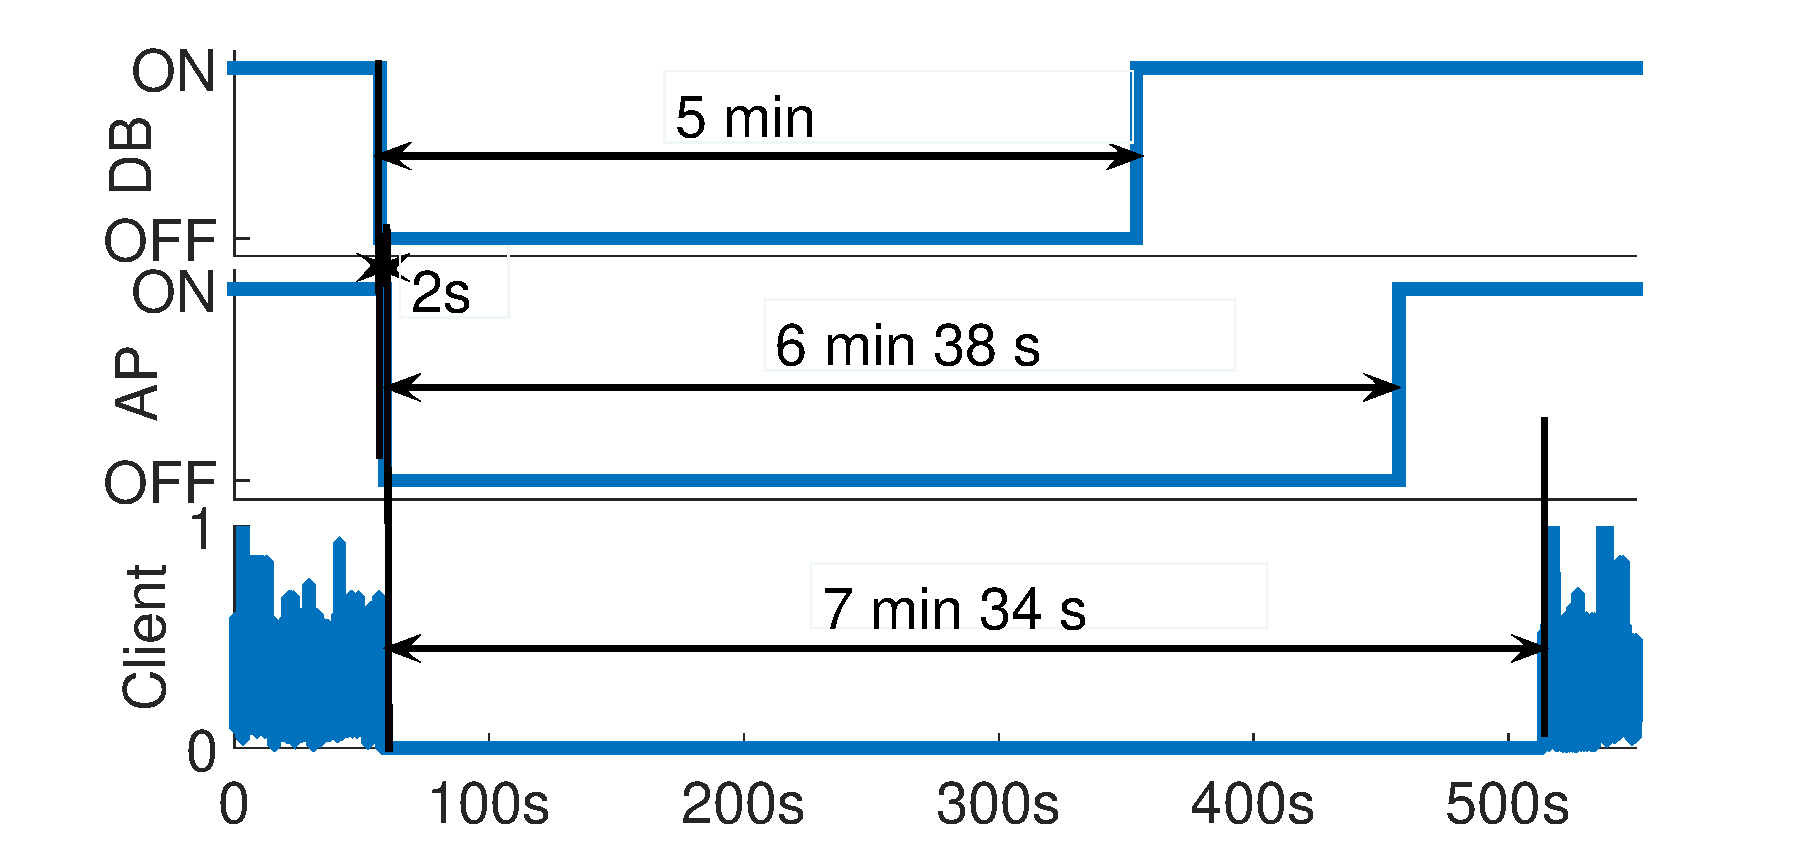
\includegraphics[width=0.5\textwidth]{./figs/paws.pdf}
  \vskip -6pt
  \caption{\small{Spectrum database interaction experiment: At 57sec channel is removed from the database for 5 min, 2 sec later the AP radio is turned off and the client stops transmitting.}}
  \label{fig:paws}
  \vskip -6pt
\end{figure}

%We see that 2sec after the channel has been removed, the radio is off. The client stops transmitting at the same time. This is well below the 60sec ETSI \cite{etsi_tvws} requirement. 

AP takes 1min 36sec to reboot and start the radio after channel is reintroduced. This is because our interface with the AP requires an AP reboot after any radio parameter changes. We note that this process can be shortened using more advanced AP control interfaces such as TR-069~\cite{tr69}. 

Once the AP is on, it takes another 56s for a client to connect and resume traffic because it has to perform cell search on various frequencies in multiple LTE bands. This time can be further reduced by disabling unused LTE bands, which we are unable to do on our existing clients. 

\begin{figure*}[htb!]
  \hfill
  \begin{minipage}{0.15\textwidth}
    \centering
    (a)
    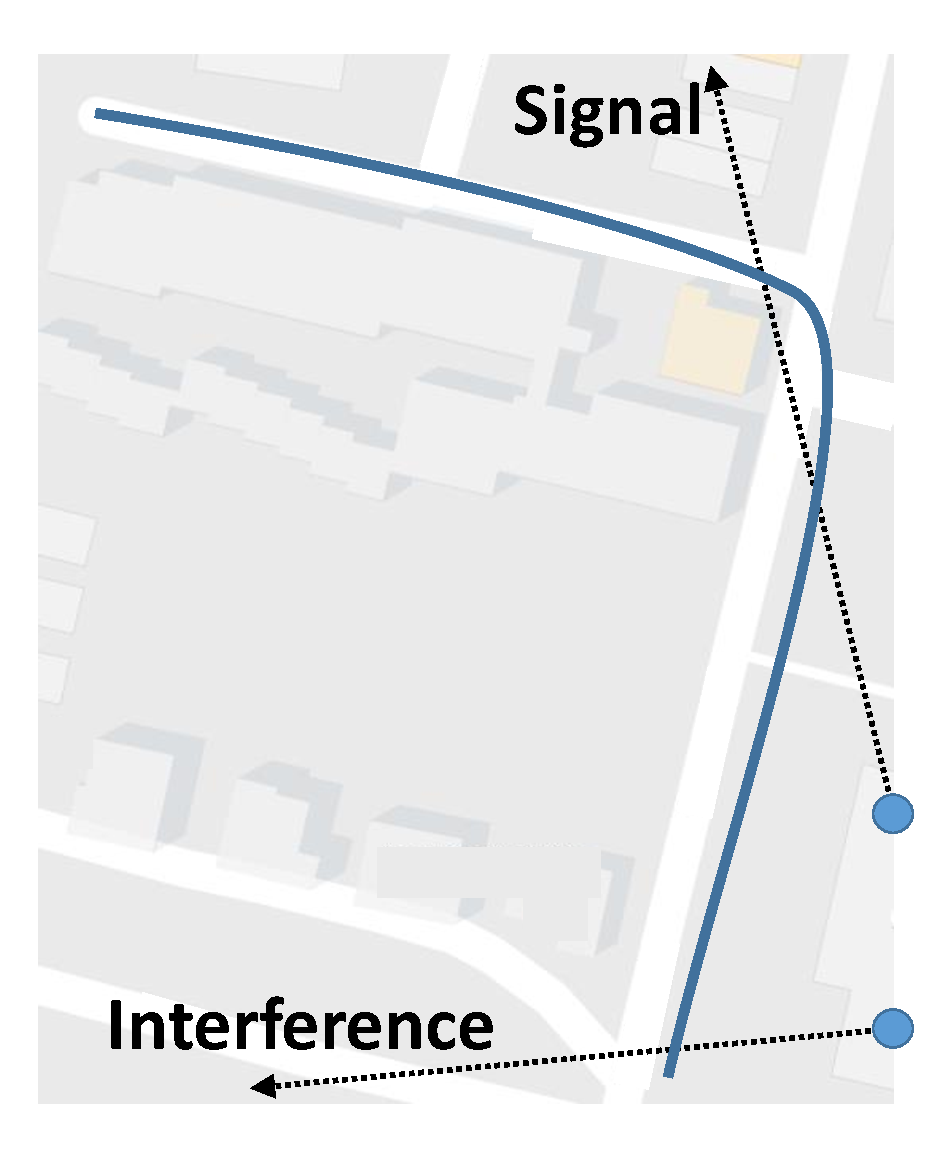
\includegraphics[width=\textwidth]{./figs/outdoor.pdf}
  \end{minipage}
  \hspace{12pt}
  \begin{minipage}{0.4\textwidth}
    \centering
    (b)
    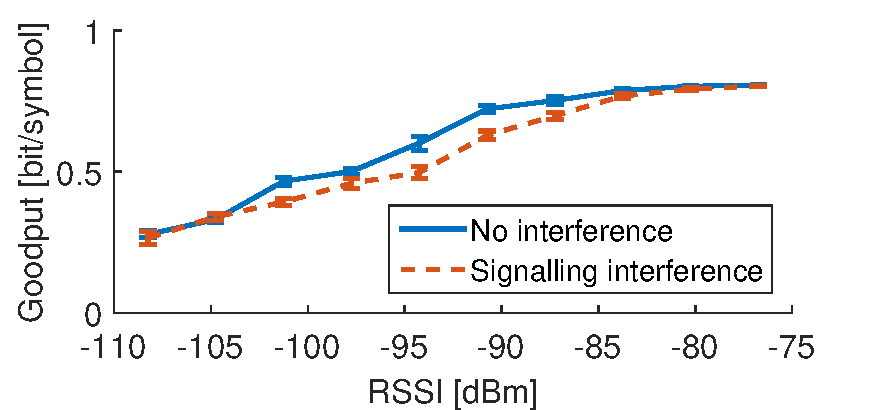
\includegraphics[width=\textwidth]{./figs/sig_vs_no.pdf}
  \end{minipage}
  \begin{minipage}{0.4\textwidth}
    \centering
    (c)
    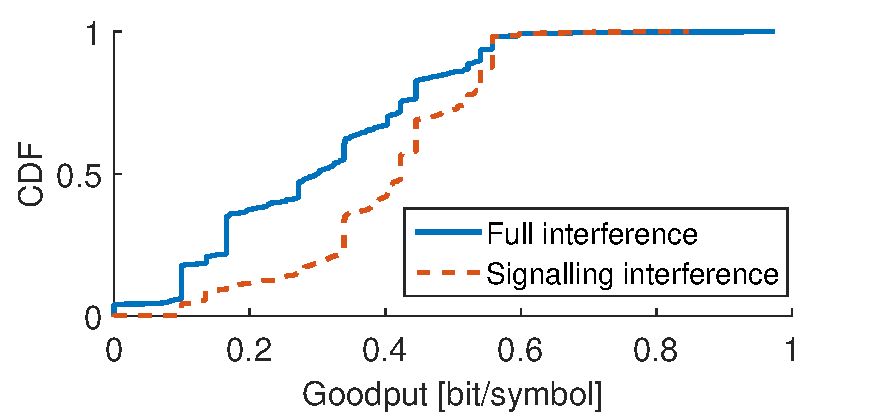
\includegraphics[width=\textwidth]{./figs/sig_vs_int.pdf}
  \end{minipage}
  \hfill
  \caption{Outdoor LTE interference experiment setup (a), 
  the difference between no interference and signalling-only interference (b) 
  and the difference between signalling-only interference and data interference (c).}
  \label{fig:interf_control}
\vskip -6pt
\end{figure*}



\subsection{Interference management}
\label{sec:interfeval}

As discussed in Section~\ref{sec:implementation}, we are unable to implement the interference management component due to software limitations of our small cell. Instead, we evaluate its key building blocks in a test-bed, and its network-level performance in large-scale simulations.



%% Second, we examine the effect of signaling and control channel interference on our design. 
%% Third, we examine whether CQI reports provide an accurate indicator of channel quality. 
%% Finally, we implement a PRACH detector using our software-defined radio to evaluate its complexity.


%\subsubsection{Signaling and control channel interference}
\subsubsection{Interference management with subchannels}

Interfering cells can mitigate inter-cell interference by avoiding to use the same subchannels at the same time.
This is not immediately obvious as LTE control elements are always present and can create interference 
even when there is no data being transmitted. This is particularly pertinent when a client is closer to an interfering cell than its serving cell. 

To understand the impact of control channel interference, we perform outdoor experiments with two E40 small cells, one acting as a serving cell and the other as an interfering one. 
The deployment is depicted in Figure~\ref{fig:interf_control}(a). 
Both cells are placed on the rooftop of our building, 15m high. The dashed lines depict the direction of each of the two antennas, and the solid blue line depicts the path over which we walked with a mobile device and performed the measurements. The end of the path is at about 250m from our building. We note that we have walked even further but due to the topology of the area the signal remains stronger than the interference and the results were similar to the ones at the end of the current path. We observe a large variability in SINR values, from -15dB to +30dB. We get such low SINR values because one end of the path is in the direction of the interference and outside of the main direction of the serving cell antenna.

We measure performance using Qualcomm's QXDM tool at the client and we log the received signal levels (RSSI) from one or both cells and the client's goodput in bits per symbol, where 
$ \mbox{bit}/\mbox{symbol} = \mbox{coding rate} \times (1-\mbox{BLER})$. 
We express goodput in bits per symbol rather than application-level throughput because our cell serves other users as well; hence, we measure throughput only within the resource blocks allocated to the test client.

We perform three measurements on the client's performance on the path: i) when only the serving cell is active, ii) when the interfering cell is active but has no users and iii) with the interfering cell being 
fully backlogged downstream. 
%first measure the client's performance on the path when only the serving cell is active. 
%In the second experiment we measure the client's performance on the same path when the interfering cell is active but has no users, hence it only emits control signals, creating control channel interference. In the third experiment we attach a user to the interfering cell and create a fully backlogged downlink. 
Figure~\ref{fig:interf_control}(b) shows the goodput as a function of the received signal strength for the case of no interference and signalling interference. The two vary by at most 20\% and in most cases much less than that. 
Hence, the control channel interference on its own does not affect the performance of data transmission significantly, even with SINR as low as -15dB. 
Figure~\ref{fig:interf_control}(c) presents the CDFs of the achieved goodputs with control channel interference only and with full data interference. 
We consider only the points where SINR is below 10dB, as in the other cases the goodput does not get affected much. We see that data interference can reduce the throughput by as much as 50\% in some cases. 
Also, we observe frequent disconnects at one end of the path when data interference is present, which we don't observe with control channel interference 
(disconnections are not included in the figure as we cannot register goodput during these intervals). 

Overall, data interference is critical in an LTE system.
Yet, two cells can share the spectrum successfully if they can coordinate data access in a way that we propose in Section~\ref{sec:archint}, despite interference from the control plane. 
We use these measurement results in our simulations to account for the effects of control-channel interference. 




\subsubsection{CQI \& channel quality}
\label{sec:eval_cqi}

The distributed subchannel selection algorithm is based on detecting subchannel interference from CQI reports (Section~\ref{sec:sensing}). 
We now demonstrate that CQI is a sufficiently accurate estimator of interference. 

Our CQI estimator needs to balance two challenges. First, channel quality fluctuates due to changes in the environment.
Second, an interfering signal might be weakened due to fading and not affect the overall throughput. 
The estimator should not trigger subchannel reallocation due to mis-identification of interference or when 
the interference signal is weak as this could result in loss of throughput; this will not allow the network to converge. 
These effects are highlighted through real measurements in Figure~\ref{fig:interf_control_time}. 
Due to fluctuating channel conditions, throughput varies significantly in the second OFF period, even when no interference is present.
Further, the last ON period shows the effect of fading, where despite interference being present, its signal is weak thus not affecting the overall throughput.

While \cf requires subband CQI reporting, our commercial small-cell access point does not implement the full LTE spec 
and only reports wide-band CQI over the entire 5 MHz channel. Thus, we only use wideband CQI reporting for this experiment. 
Yet, the same observations apply.

Our estimator works as follows. Since interference is typically bursty, we consider the maximum CQI observed within a time window as an estimate of CQI for a channel without interference. 
We declare that interference is present if we observe a CQI report below 60\% of this maximum value over a window of 10 consecutive samples. 
We measure the false positives by running the detector over samples of the channel without interference. 
We observe that it has less than 2\% false positives, i.e., one false positive every 100ms on average
(CQI is sampled every 2 ms). 
Our measurements further show that when interference is strong, our detector correctly reports interference with 80\% probability.
As with the interference measurements, we use these results in our simulations to model imperfect interference detection. 

%% Figure~\ref{fig:cqi} presents the accuracy of the estimator when interference is present, as a function of the level of interference.
%% The figure shows that when interference is strong, our detector correctly reports interference with 80\% probability.

\begin{figure}[t]
\vspace{-10pt}
  \centering
    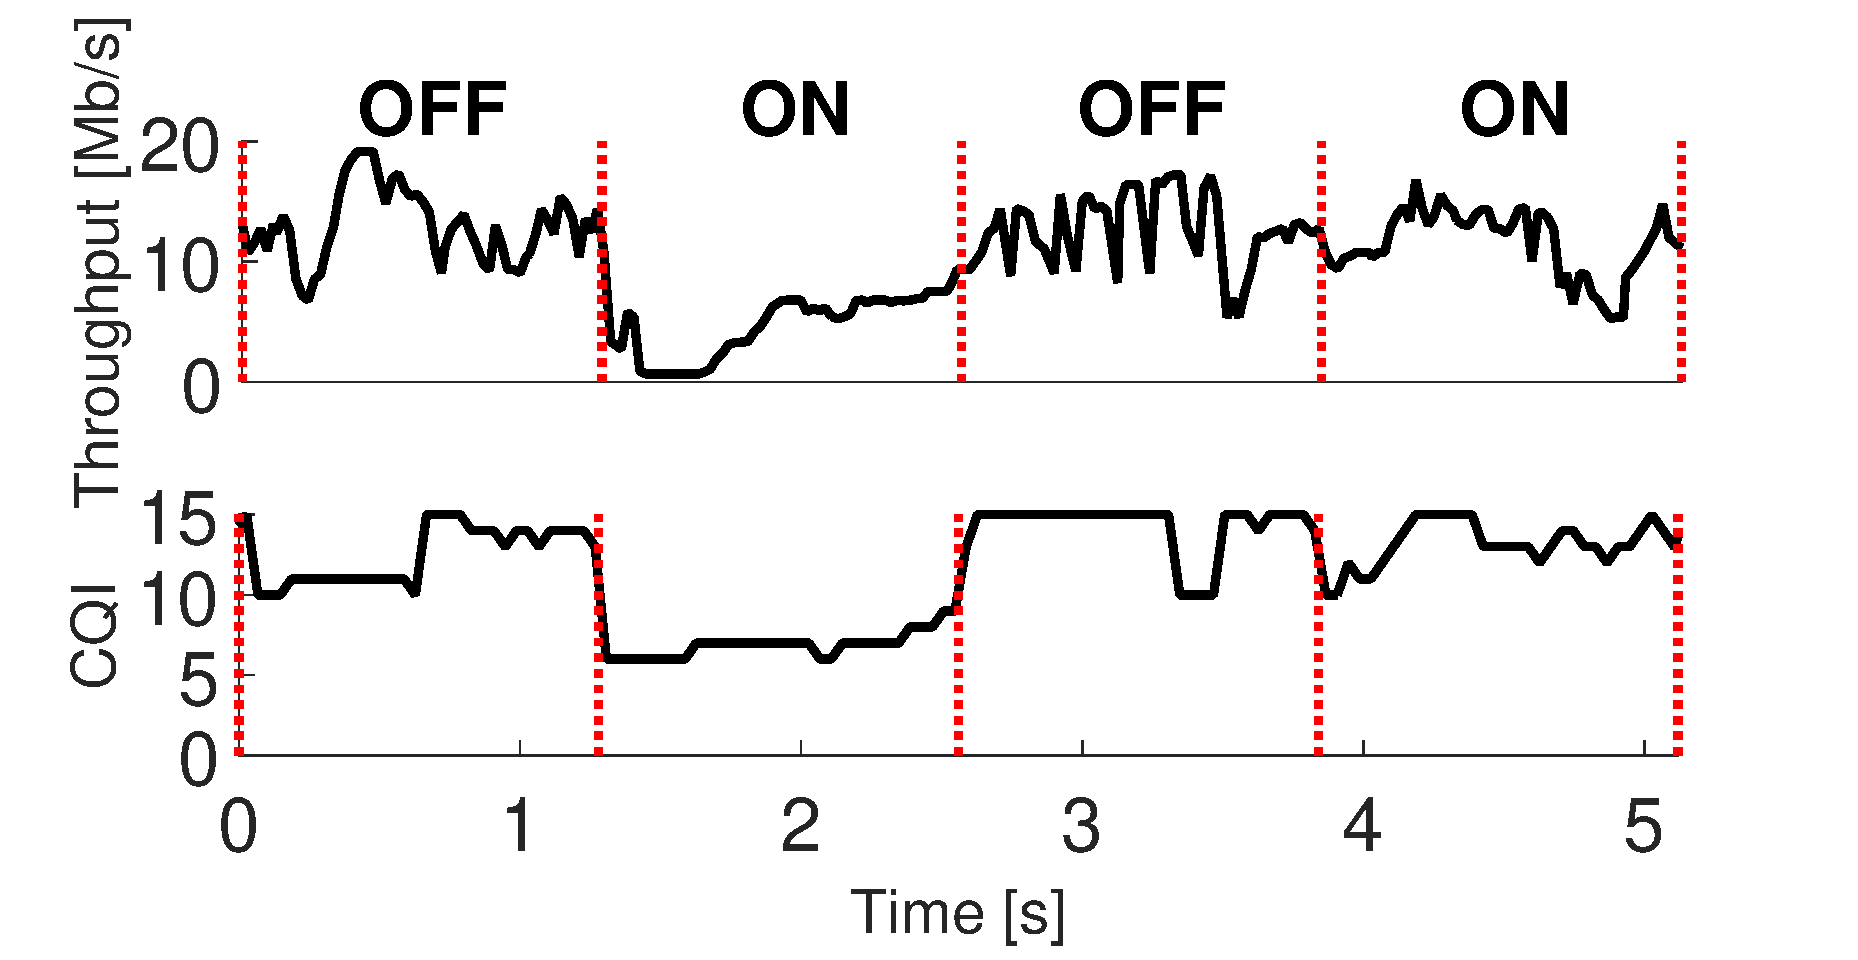
\includegraphics[width=0.38\textwidth]{./figs/cqi_time.pdf}
    \vspace{-0.15in}
  \caption{\small{PHY throughput and channel quality indicator (CQI) reported during four states of interfering radio. 
ON denotes times where there is interference. }}
\vspace{-0.22in}

  \label{fig:interf_control_time}
\end{figure}

%% \begin{figure}[t]
%%   \centering
%%     \includegraphics[width=0.5\textwidth, height=0.4\columnwidth]{./figs/CQI.pdf}
%%     \vspace{-0.3in}
%%   \caption{Channel quality indicator (CQI) detection vs. the relative rate of interference.}
%%   \label{fig:cqi}
%% \end{figure}




\subsubsection{PRACH preamble detection}
\label{sec:pracheval}

\cf uses PRACH to estimate the number of contending clients. 
It is known that PRACH preambles can be detected at -10dB~\cite{prach}.
Here, we show that we can design a low-complexity PRACH detector for that purpose.


%% Clients initiate connections by sending PRACH preambles to access points they are associated with at predefined time instants. 
%% The main parameter of a PRACH signal is a preamble sequence number. 
%% The PRACH waveform is created from a root sequence using a cyclic shift that 
%% corresponds to the preamble sequence number. 
%% The sequence number is chosen randomly by clients for each PRACH transmission, 
%% and is used by access points to resolve potential contention among multiple clients~\cite{LTEbullets}. 

The key challenge for an access point trying to overhear PRACH preambles from clients not associated with it, 
is detecting these preambles efficiently without knowing the preamble sequence number~\cite{LTEbullets} or having the timing information. 
A naive implementation would correlate several long PRACH sequences, one for each preamble sequence number, 
whenever new samples are received. 

We propose a different detector which leverages the structure of the preambles. 
If we correlate a PRACH preamble received with a time offset, it will have a cyclic shift in its frequency representation. 
Equally, a different cyclic shift will be caused by a different preamble sequence number. 
We only need to detect whether a preamble is present, and neither need to know which preamble sequence has been transmitted 
nor when the transmission has started. 
Thus, we only need to perform two correlations; one to detect the most likely cyclic shift and 
another to check its correlation value. 

We implemented the modified detector on the SDR platform.
The detector has a comparable performance to a conventional implementation (with timing information) 
when receiving PRACH signals from a commercial dongle. 
Overall, it is 16 times faster than the required line rate (when ran on an Intel i7 CPU on a 10MHz channel).





